%%%%%%%%%%%%%%%%%%%%%%%%%%%%%%%%%%%%%%%%%
% Masters/Doctoral Thesis 
% LaTeX Template
% Version 2.5 (27/8/17)
%
% This template was downloaded from:
% http://www.LaTeXTemplates.com
%
% Version 2.x major modifications by:
% Vel (vel@latextemplates.com)
%
% This template is based on a template by:
% Steve Gunn (http://users.ecs.soton.ac.uk/srg/softwaretools/document/templates/)
% Sunil Patel (http://www.sunilpatel.co.uk/thesis-template/)
%
% Template license:
% CC BY-NC-SA 3.0 (http://creativecommons.org/licenses/by-nc-sa/3.0/)
%
%%%%%%%%%%%%%%%%%%%%%%%%%%%%%%%%%%%%%%%%%

%----------------------------------------------------------------------------------------
%	PACKAGES AND OTHER DOCUMENT CONFIGURATIONS
%----------------------------------------------------------------------------------------

\documentclass[
11pt, % The default document font size, options: 10pt, 11pt, 12pt
%oneside, % Two side (alternating margins) for binding by default, uncomment to switch to one side
english, % ngerman for German
singlespacing, % Single line spacing, alternatives: onehalfspacing or doublespacing
%draft, % Uncomment to enable draft mode (no pictures, no links, overfull hboxes indicated)
%nolistspacing, % If the document is onehalfspacing or doublespacing, uncomment this to set spacing in lists to single
%liststotoc, % Uncomment to add the list of figures/tables/etc to the table of contents
%toctotoc, % Uncomment to add the main table of contents to the table of contents
parskip, % Uncomment to add space between paragraphs
%nohyperref, % Uncomment to not load the hyperref package
headsepline, % Uncomment to get a line under the header
%chapterinoneline, % Uncomment to place the chapter title next to the number on one line
%consistentlayout, % Uncomment to change the layout of the declaration, abstract and acknowledgements pages to match the default layout
]{MastersDoctoralThesis} % The class file specifying the document structure

\usepackage[utf8]{inputenc} % Required for inputting international characters
\usepackage[T1]{fontenc} % Output font encoding for international characters

\usepackage{mathpazo} % Use the Palatino font by default
\usepackage{amsmath}

\usepackage[backend=bibtex,style=numeric ,natbib=true]{biblatex} % Use the bibtex backend with the authoryear citation style (which resembles APA)

\addbibresource{example.bib} % The filename of the bibliography

\usepackage[autostyle=true]{csquotes} % Required to generate language-dependent quotes in the bibliography

%----------------------------------------------------------------------------------------
%	MARGIN SETTINGS
%----------------------------------------------------------------------------------------

\geometry{
	paper=a4paper, % Change to letterpaper for US letter
	inner=2.5cm, % Inner margin
	outer=3.8cm, % Outer margin
	bindingoffset=.5cm, % Binding offset
	top=1.5cm, % Top margin
	bottom=1.5cm, % Bottom margin
	%showframe, % Uncomment to show how the type block is set on the page
}

%----------------------------------------------------------------------------------------
%	THESIS INFORMATION
%----------------------------------------------------------------------------------------

\thesistitle{Thesis Title} % Your thesis title, this is used in the title and abstract, print it elsewhere with \ttitle
\supervisor{Dr. James \textsc{Smith}} % Your supervisor's name, this is used in the title page, print it elsewhere with \supname
\examiner{} % Your examiner's name, this is not currently used anywhere in the template, print it elsewhere with \examname
\degree{Doctor of Philosophy} % Your degree name, this is used in the title page and abstract, print it elsewhere with \degreename
\author{John \textsc{Smith}} % Your name, this is used in the title page and abstract, print it elsewhere with \authorname
\addresses{} % Your address, this is not currently used anywhere in the template, print it elsewhere with \addressname

\subject{Biological Sciences} % Your subject area, this is not currently used anywhere in the template, print it elsewhere with \subjectname
\keywords{} % Keywords for your thesis, this is not currently used anywhere in the template, print it elsewhere with \keywordnames
\university{\href{http://www.university.com}{University Name}} % Your university's name and URL, this is used in the title page and abstract, print it elsewhere with \univname
\department{\href{http://department.university.com}{Department or School Name}} % Your department's name and URL, this is used in the title page and abstract, print it elsewhere with \deptname
\group{\href{http://researchgroup.university.com}{Research Group Name}} % Your research group's name and URL, this is used in the title page, print it elsewhere with \groupname
\faculty{\href{http://faculty.university.com}{Faculty Name}} % Your faculty's name and URL, this is used in the title page and abstract, print it elsewhere with \facname

\AtBeginDocument{
\hypersetup{pdftitle=\ttitle} % Set the PDF's title to your title
\hypersetup{pdfauthor=\authorname} % Set the PDF's author to your name
\hypersetup{pdfkeywords=\keywordnames} % Set the PDF's keywords to your keywords
}


\begin{document}

\frontmatter % Use roman page numbering style (i, ii, iii, iv...) for the pre-content pages

\pagestyle{plain} % Default to the plain heading style until the thesis style is called for the body content

%----------------------------------------------------------------------------------------
%	TITLE PAGE
%----------------------------------------------------------------------------------------'
%\begin{titlepage}
%\begin{center}
%
%\vspace*{.06\textheight}
%{\scshape\LARGE \univname\par}\vspace{1.5cm} % University name
%\textsc{\Large Doctoral Thesis}\\[0.5cm] % Thesis type
%
%\HRule \\[0.4cm] % Horizontal line
%{\huge \bfseries \ttitle\par}\vspace{0.4cm} % Thesis title
%\HRule \\[1.5cm] % Horizontal line
% 
%\begin{minipage}[t]{0.4\textwidth}
%\begin{flushleft} \large
%\emph{Author:}\\
%\href{http://www.johnsmith.com}{\authorname} % Author name - remove the \href bracket to remove the link
%\end{flushleft}
%\end{minipage}
%\begin{minipage}[t]{0.4\textwidth}
%\begin{flushright} \large
%\emph{Supervisor:} \\
%\href{http://www.jamessmith.com}{\supname} % Supervisor name - remove the \href bracket to remove the link  
%\end{flushright}
%\end{minipage}\\[3cm]
% 
%\vfill
%
%\large \textit{A thesis submitted in fulfillment of the requirements\\ for the master degree of \degreename}\\[0.3cm] % University requirement text
%\textit{in the}\\[0.4cm]
%\groupname\\\deptname\\[2cm] % Research group name and department name
% 
%\vfill
%
%{\large \today}\\[4cm] % Date
%\includegraphics{Logo} % University/department logo - uncomment to place it
% 
%\vfill
%\end{center}
%\end{titlepage}

%----------------------------------------------------------------------------------------
%	DECLARATION PAGE
%----------------------------------------------------------------------------------------

%\begin{declaration}
%\addchaptertocentry{\authorshipname} % Add the declaration to the table of contents
%\noindent I, \authorname, declare that this thesis titled, \enquote{\ttitle} and the work presented in it are my own. I confirm that:
%
%\begin{itemize} 
%\item This work was done wholly or mainly while in candidature for a research degree at this University.
%\item Where any part of this thesis has previously been submitted for a degree or any other qualification at this University or any other institution, this has been clearly stated.
%\item Where I have consulted the published work of others, this is always clearly attributed.
%\item Where I have quoted from the work of others, the source is always given. With the exception of such quotations, this thesis is entirely my own work.
%\item I have acknowledged all main sources of help.
%\item Where the thesis is based on work done by myself jointly with others, I have made clear exactly what was done by others and what I have contributed myself.\\
%\end{itemize}
% 
%\noindent Signed:\\
%\rule[0.5em]{25em}{0.5pt} % This prints a line for the signature
% 
%\noindent Date:\\
%\rule[0.5em]{25em}{0.5pt} % This prints a line to write the date
%\end{declaration}
%
%\cleardoublepage

%----------------------------------------------------------------------------------------
%	QUOTATION PAGE
%----------------------------------------------------------------------------------------

\vspace*{0.2\textheight}

\noindent\enquote{\itshape Thanks to my solid academic training, today I can write hundreds of words on virtually any topic without possessing a shred of information, which is how I got a good job in journalism.}\bigbreak

\hfill Dave Barry

%----------------------------------------------------------------------------------------
%	ABSTRACT PAGE
%----------------------------------------------------------------------------------------

\begin{abstract}
\addchaptertocentry{\abstractname} % Add the abstract to the table of contents
In this report, we investigate the stochastic local volatility (SLV) model for derivative contracts on commodity futures. Means of simulation and parsimonious parametrisation are considered to deal with the limited quotes in the market. First, the report considers a scheme of extracting normalised call prices from market quotes by an extensive Dupire equation together with the implied volatility. Then we proceed to the calibration of the local volatility model including the calibration of the mean-reversion speed. Next, a pricing mechanism is developed with the backward PDE methods or an iterative Monte-Carlo simulations of the local volatility surface. Finally, we evaluate the performance of the model on market data.\ldots
\end{abstract}

%----------------------------------------------------------------------------------------
%	ACKNOWLEDGEMENTS
%----------------------------------------------------------------------------------------

\begin{acknowledgements}
\addchaptertocentry{\acknowledgementname} % Add the acknowledgements to the table of contents
The acknowledgments and the people to thank go here, don't forget to include your project advisor\ldots
\end{acknowledgements}

%----------------------------------------------------------------------------------------
%	LIST OF CONTENTS/FIGURES/TABLES PAGES
%----------------------------------------------------------------------------------------

%\tableofcontents % Prints the main table of contents
%
%\listoffigures % Prints the list of figures
%
%\listoftables % Prints the list of tables
%
%----------------------------------------------------------------------------------------
%	ABBREVIATIONS
%----------------------------------------------------------------------------------------

%\begin{abbreviations}{ll} % Include a list of abbreviations (a table of two columns)
%
%\textbf{LAH} & \textbf{L}ist \textbf{A}bbreviations \textbf{H}ere\\
%\textbf{WSF} & \textbf{W}hat (it) \textbf{S}tands \textbf{F}or\\
%
%\end{abbreviations}
%
%----------------------------------------------------------------------------------------
%	PHYSICAL CONSTANTS/OTHER DEFINITIONS
%----------------------------------------------------------------------------------------

%\begin{constants}{lr@{${}={}$}l} % The list of physical constants is a three column table
%
%% The \SI{}{} command is provided by the siunitx package, see its documentation for instructions on how to use it
%
%Speed of Light & $c_{0}$ & \SI{2.99792458e8}{\meter\per\second} (exact)\\
%%Constant Name & $Symbol$ & $Constant Value$ with units\\
%
%\end{constants}
%
%----------------------------------------------------------------------------------------
%	SYMBOLS
%----------------------------------------------------------------------------------------

%\begin{symbols}{lll} % Include a list of Symbols (a three column table)
%
%$a$ & distance & \si{\meter} \\
%$P$ & power & \si{\watt} (\si{\joule\per\second}) \\
%%Symbol & Name & Unit \\
%
%\addlinespace % Gap to separate the Roman symbols from the Greek
%
%$\omega$ & angular frequency & \si{\radian} \\
%
%\end{symbols}

%----------------------------------------------------------------------------------------
%	DEDICATION
%----------------------------------------------------------------------------------------

\dedicatory{For/Dedicated to/To my\ldots} 

%----------------------------------------------------------------------------------------
%	THESIS CONTENT - CHAPTERS
%----------------------------------------------------------------------------------------

\mainmatter % Begin numeric (1,2,3...) page numbering

\pagestyle{thesis} % Return the page headers back to the "thesis" style

% Include the chapters of the thesis as separate files from the Chapters folder
% Uncomment the lines as you write the chapters

% Chapter 1

\chapter{Introduction} % Main chapter title

\label{Chapter1} % For referencing the chapter elsewhere, use \ref{Chapter1} 

%----------------------------------------------------------------------------------------

% Define some commands to keep the formatting separated from the content 
\newcommand{\keyword}[1]{\textbf{#1}}
\newcommand{\tabhead}[1]{\textbf{#1}}
\newcommand{\code}[1]{\texttt{#1}}
\newcommand{\file}[1]{\texttt{\bfseries#1}}
\newcommand{\option}[1]{\texttt{\itshape#1}}

%----------------------------------------------------------------------------------------
\section{Commodity Market Overview}
Commodity trading is as old as civilisation. It is believed that the first commodity market can be long dated back to between 4500 and 4000 BC in Sumer. Sumerians used clay writing tablets to document the amount of goods and delivery date of the trade. This ancient trading system reassembles to today's futures contracts in commodity market. Medieval Europe saw a prosperous growth in Commodity market, with the first stock exchange established in Amsterdam in 1530 which also operated as a market for the exchange of commodities. Nowadays, the commodity trading is no longer restricted to the physical format. In fact, among over 50 major commodities exchanges worldwide, purely financial transactions has been increasingly outnumbering physical trades particularly in energy market. 

A commodity market is referred to a physical or virtual platform that trades in primary economic sector. Modern commodity trading includes the form of spot trading and derivative trading. In spot trading market, physical delivery of goods and payment are involved between the market participants. The prices in this market is a reflection of the current or very near term market equilibrium of demand and supply. 

The derivatives market, on the other hand, provides trading platform of derivative contracts written on the spot price. These derivatives take form of forwards, futures and options on futures with futures being the most traded one. Commodity features prices reflect a collective review from both buy side and sell side of the future market supply and demand. Commodity derivatives are secured by physical assets or commodities. Hence unlike bonds and stocks, commodities are valued not based on the profitability or cash flows but rather on the estimated future prices implied by the market demand and supply of the physical item. Due to this nature, commodity market remains the most volatile asset class. Crude oil has seen quarterly volatility surge from 12.63\% to over 90\% since 1983. During financial crisis, in particular, the price crashed almost 500\% in less than half a year--the WTI crude oil prices reached its peak of US\$147.27 on 11 July 2008 and fell to US\$30.28 a barrel on 23 December the same year. Even more evidently, the price of WTI crude oil features contract plunged into negative in May 2020 settled at US-\$37.63 a barrel for the first time in history due to the Covid-19. Similar examples include: 1970's oil crises\parencite{olicrises}and 1980's oil glut\parencite{oliglut}. This reflects the fact that alongside with mother nature, geopolitics and speculations also influence the global demand and supply of commodities greatly. Because of the volatile nature of the commodity, many institutional users of commodities confronted with rising raw material prices may wish to lock in low prices to avoid risks in future prices. Airline companies, for example, secure a massive amount of fuels at a reasonable price by entering a future contract.  A future contract is a standardised legal agreement to buy or sell a commodity at a predetermined price often with agreed quantity and quality and a specific time in the futures. At this future date, either physical delivery of the commodity or cash settlement will take place. In practice, physical delivery only occurs in a minority of contracts since it can be very costly taking into account the delivery and storage expense. Most commodity futures traders often offset their contracts before expiry date. This is normally done by purchasing a covering position, Nymex crude futures contract uses this method of settlement upon expiration. To maintain the same risk position beyond the initial expiration, some traders also choose to roll over the contract--switch from the near expiration contract to one further-out month. The original contract has to be closed meaning that the loss or gain is required to be settled before entering into a new one. In case of physical delivery, the position has to be closed before first notification date and last notification date for a cash settled contract. 

Many financial futures based on market indexes are cash settled, for example, the popular E-minis which track the S\&P 500 market index was launched in 1997 and traded on the Chicago Mercantile Exchange (CME) via their Globex electronic trading platform. Cash settled futures contracts are preferred by a lot of the investors with its two major advantages\parencite{lien_tse_2002}. First, a cash settled contract ensures the convergence between spot price and futures price at expiration which enhances its power as a hedging instrument. Second, cash settlement reduces the market manipulation such as cornering and squeezing.  

Commodity market has continued gaining traction in the recent decades, many portfolio managers add commodity derivatives as an asset class. Basu and Gavin\parencite{basu_gavin_2011} proposed two possible explanations for the surge in trading commodity derivatives. With first one being greater appetite for risky asset in general and the second explanation is a mistaken notion that an investment in commodity futures can be used to hedge equity risk.



%----------------------------------------------------------------------------------------








\subsection{Market Convention}
Commonly traded commodities are split into four categories: energy, metal, livestock and meat, Agriculture. Energy commodities include crude oil, heating oil, natural gas, and gasoline. Prices of crude oil is extremely sensitive to consumer and investor sentiment. As such the crude oil market is very volatile to geopolitics and extreme climate. With West Texas Intermediate (WTI) and Brent North Sea Crude(Brent Crude) being the most popular traded ones on the market, Brent crude's price is the benchmark for African, European, and Middle Eastern crude oil, while WTI is he benchmark for North America. The futures contracts of WTI are listed on New York Mercantile Exchange (NYMEX) and the physical delivery happens in Cushing, Oklahoma\parencite{cme_future}.  Brent crude oil futures trade on the Intercontinental Exchange (ICE) and are traded globally with various delivery locations around the world. Both Brent Crude and WTI has a contract size with 1,000 barrels, with 134 maximum contracts for WTI and 96 for Brent Crude in the futures contract series are available for trading. 
Physical delivery often takes forms of inter-facility transfer through pipeline, in-line transfer or in-tank transfer where the crude oil remains physically stationary but the title is transferred. 


Metals are another important resources for production and investment purpose next to crude oil. The precious metals with active markets include: gold, silver, platinum.  Investors tend to invest in precious metals during time of market market volatility and uncertainty or period of high inflation to mitigate the risk. The three main factors in the metal market are: demand from China, technological  innovations and  institutional regulations. S\&P GSCI Precious Metals Index( \string^ SPGSI), S\&P GSCI Industrial Metals Select( \string^ SPGSINP) and UBS Bloomberg CMCI Industrial Metals Index Total Return ( \string^ UBM-SO).

The difference between spot and futures prices is generally called the basis. When the spot price is higher than the futures price, it is called backwardation, and when it is lower it is called contango. Backwardation and contango are also used to describe the relationship between two futures contracts of the same commodity.







\subsection{Motivation}
Increased volatility of commodity prices add great risk to economy and investment. For commodity investors, changing in price directly affects the \textit{marginal convenience yield}, an adjustment to the cost of carry in forward pricing formula under non-arbitrage argument which make backwardation pronounce. Secondly, price volatilities also increase the \textit{option premium}, i.e the opportunity cost of exercising the option instead of holding up for more information\parencite{pindyck}. This opportunity cost reinforces the backwardation in the first effect we listed\parencite{litzenberger}. 

Volatility dynamics are a key consideration in strategy formation for hedging, derivatives
trading, and portfolio optimisation. Commodity futures, in particular, add a valuable source of diversification benefits compared to traditional assets class for investors and portfolio managers. Because the futures market is highly liquid and volatile, derivatives on futures price have also gained more tractions. However, many trades and investments decisions in commodity derivatives market are not made under a correct pricing scheme. Especially for customised derivative contracts that are illiquid, opaque, or have little market depth or limited expirations, a pricing model for future prices that incorporates both the forward curve and smile dynamic is required. Such a model provide an accurate price discovery, option modelling and risk management for investors. In addition, a comprehensive understanding and modelling of futures dynamic also enables policy makers to re-evaluate the adequacy of current regulations and interventions to better improve the social welfare. 


\subsection{Objective}
This thesis concerns two closely related objectives. The first objective is to propose a method to simulate realistic futures price and quoted option prices on commodity market. Secondly, to present stochastic-local volatility model which incorporates both forward-curve and smile dynamics of the volatility. 







%-----------------------------------------------------------
\subsection{Methodology and Outline}


 
%----------------------------------------------------------------------------------------





%----------------------------------------------------------------------------------------



%----------------------------------------------------------------------------------------



%% Chapter Template

\chapter{Literature Review} % Main chapter title

\label{Chapter2} % Change X to a consecutive number; for referencing this chapter elsewhere, use \ref{ChapterX}

%----------------------------------------------------------------------------------------
%	SECTION 1
%----------------------------------------------------------------------------------------

\section{Existing Literature }
Earlier studies on commodity market focus on price discovery. One dimensional model that assumes Brownian motion and constant convenience rate was first developed by Merton~\parencite{} in early 70's, followed by a series of mean reverting models which considered as better price forecaster. Popular models included Geometric Ornstein-Uhlenbeck model by Dixit and Pindyck~\parencite{dixit1994} which has an additional drift term to revert the price back to equilibrium level. Some models are further developed to include a convenience yield as a stochastic state such as in Gibson and Schwartz\parencite{Gibson1990}, where the parameters are estimated by weekly futures price. Later, Schwartz and Smith\parencite{smith2000} modified it to a two factor model that captures both long term mean and short term fluctuations in the prices. The long term mean is assumed to follow a geometric brownian motion with a drift term reflecting current market situation, and the short time derivation is modelled by an Ornstein-Uhlenbeck process. Due to the poor fitting of two factor models on commodity futures with longer maturity as well as the growing liquidity of longer maturity contracts, a three factor model is proposed again by Schwartz in 1997 under stochastic connivence and instantaneous interest rate following a mean reverting process as in Vasicek model~\parencite{vasicek1977}. Risk premia 
are assumed to be constant, parameters are extracted from historical data and through Kalman filter. More developments on the three factor model can be seen in paper by Hilliard and Reis~\parancite{hilliard_reis_1998} where the underlying spot prices follow a jump diffusion process~\parencite{bates1991} with non-zero mean jump to allow large discrete jumps. In addition, an equilibrium connivence yield diffusion and an arbitrage free interest rate diffusion are assumed. These models mentioned above seek to model the evolution of spot prices and then price the futures under the arbitrage free framework, finally the forward curve is derived from the future process. Because of the spot price are traditional observable and the most liquid, we adopt the same approach to model the forward curve and smile of volatility in commodity market and hence produce the feature prices and option prices quoted on futures. We follow the work done by Pallavicini~\parencite{Pallavicini2018} at el in which a local-volatility one-factor mean reverting process with affine drift is defined to model marginal density of the future prices and then a quick and robust calibration algorithm to all quoted options. Additionally, a stochastic local volatility dynamic is introduced to allow forward curve and smile structure for each future. The advantage of this model compared to traditional multi-factor stochastic volatility model is that the calibration is quick and robust such that it is applicable to partitioners on trading desks.
%-----------------------------------
%	SUBSECTION 1
%-----------------------------------
\subsection{Methodology}
The model of our interest is by Pallavicini at el.~\parencite{Pallavicini2018}. Related literature in the similar topic can be found in Pilz and Schl�gl~\parencite{}, Albani et al. \parencite{} and Chiminello~\parencite{}. However, none of them discussed 'Smile' effect related to strike prices is not discussedAmong these models, the first one considered a different stochastic process for each future price together with a designated  local volatility factor. Stochastic interest rates are incorporated for the forward structure in the futures prices. The second model introduces a distinct local volatility for each future price and a complete set of option quotes is simulated from existing ones to facilitate the calibration process. The last model considers a class of local volatility surfaces and assumes the future prices are diffusion process driven by such volatility surface without drift. In this report we adopt the the model described in \parencite{Pallavicini2018}. We define a two-step  calibration procedure. First, we introduce a linear local volatility model with an affine drift term~\parencite{} to model the spot prices. The future prices are then readily available in a closed form.  Option prices and futures prices are required to calibrate the stochastic parameters in the linear model. First, we start with the calibration of the futures prices by solving a first order ODE explicitly. We then proceed to calibrate the local volatility function in the dynamics of the futures prices. To achieve a quick and robust calibration, we employ 

an iterative calibration strategy by guessing the optimal parameters based on the mismatch from the target and model implied quantity as discussed in~ \parencite{Reghai}. The last step involves the calibration of mean reversion speed in the futures prices dynamics by looking at liquid mid-curve options (MCO) or calendar spread options(CSO), similarly in the work by~\parencite{anderson}. To model the curve and skew dynamics, we look at the joint probability densities between multiple futures prices and the transition densities in each futures dynamics. In Pallavicini at el's model, they promote each futures price to follow a different SLV model, a new calibration method is developed in which a two dimensional model including the local volatility and correlation parameters is considered. The calibration of mean reversion and correlation parameters to market quotes can be
done by solving the corresponding bi-dimensional pricing PDEs. 
Finally, if we wish to also model the smile dynamics we need to introduce a stochastic volatility process as defined in \parencite{ren} with a three factor process and the calibration procedures can be derived henceforward. 
%-----------------------------------
%	SUBSECTION 2
%-----------------------------------
 
%\include{Chapters/Chapter3}
% Chapter 4

\chapter{Models Capture the Smile} % Main chapter title

\label{Chapter4} % For referencing the chapter elsewhere, use \ref{Chapter1} 
% Define some commands to keep the formatting separated from the content 
%\newcommand{\keyword}[4]{\textbf{#4}}
%\newcommand{\tabhead}[4]{\textbf{#4}}
%\newcommand{\code}[4]{\texttt{#2}}
%\newcommand{\file}[4]{\texttt{\bfseries#4}}
%\newcommand{\option}[4]{\texttt{\itshape#4}}

%----------------------------------------------------------------------------------------
Enormous body of research have been conducted on the volatility models, largely motivated by its importance in financial market. The volatility of a financial instrument is often seen as one of the most important risk indicators as well as a key parameter in many pricing models in financial market. In this section we first review local volatility (LV) models and stochastic volatility (SV) models. In the class of  local volatility models, we start with the Dupire's local volatility model which is a generalisation of the classic Black-Scholes model \parencite{bs1973} and then move to Displaced Diffusion model introduced by Rubinstein \parencite{displaced_process} which generates a sloping implied skew to the original model. Then we proceed to a class of stochastic volatility models where volatility is driven by an additional stochastic differential equation. The most popular ones among financial institutions include Heston model \parencite{Heston1993ACS} in which the randomness of the variance process varies as the square root of variance, Constant Elasticity of Variance (CEV) discussed by Cox and Ross \parencite{cox1975notes} which attempts to capture both stochastic volatility and the leverage effect.   Despite this two classes of models have the capability of capturing the smile features, they are insufficient to describe the asymptotic behaviour of the entire smile surface. This leads to the development of the stochastic local volatility (SLV) models. This class of hybrid model includes both stochastic and local volatility as its name suggests. In this model, the volatility from the stochastic volatility model can be modified with a local volatility function. Under such a construction, SLV models allow quick calibration to plain-vanilla options with the potential to extend to exotic options. 



%----------------------------------------------------------------------------------------
\section{Black-Scholes Model}
A major breakthrough in the option pricing world is made by Fisher Black and Myron Scholes \parencite{bs1973} in 1973. They developed a model for pricing a financial derivative. This model 
estimates the evolution of a price of an underlying overtime. It assumes the price of the underlying asset follows a Geometric Brownian motion under the risk-neutral measure, defined as :
\begin{equation}
\label{eqn:GBM}
dS_{t}=r S_{t}\,dt+\sigma S_{t}\,dW_{t}
\end{equation}
Where
$W_{t}$ is a Wiener process or Brownian motion,  $r$ is the risk-free rate served as 'the percentage drift' and constant volatility $\sigma$.\\

In particular, they derived a differential equation given in Equation~\ref{eqn:bls_pde} governing the price $ V(S, t)$evolution of the option under the model by applying \textit{It\^{o}}'s lemma for two variables in Equation~\ref{eqn:GBM} . 
 \begin{equation}
 \label{eqn:bls_pde}
dV=\left(\mu S{\frac {\partial V}{\partial S}}+{\frac {\partial V}{\partial t}}+{\frac {1}{2}}\sigma ^{2}S^{2}{\frac {\partial ^{2}V}{\partial S^{2}}}\right)dt+\sigma S{\frac {\partial V}{\partial S}}\,dW
\end{equation}

By solving the PDE for the corresponding terminal and boundary conditions as stated below:
\begin{align}
C(S, T) = max(S-K, 0)\\
C(0, t) = 0\\
C(\infty,t) \approx S
\end{align}
 Where $T$ is the maturity, and $K$ is the strike.
 
We have an analytic solution for European call option price given by:

 \begin{equation}
 \label{eqn:bls}
C(S_{t},t) =N(d_{1})S_{t}-N(d_{2})Ke^{-r(T-t)},
\end{equation}
with
\begin{align}
d_{1}&={\frac {1}{\sigma {\sqrt {T-t}}}}\left[\ln \left({\frac {S_{t}}{K}}\right)+\left(r+{\frac {\sigma ^{2}}{2}}\right)(T-t)\right]\\
d_{2}&=d_{1}-\sigma {\sqrt {T-t}}.
 \end{align}
where $N(x)$ denotes the standard normal cumulative distribution function

\begin{equation}
 N(x)={\frac {1}{\sqrt {2\pi }}}\int _{-\infty }^{x}e^{-z^{2}/2}\,dz.
\end{equation}
Specifically, $N(d_2)$ is the probability that the call will be exercised under the assumption that the underlying asset has the risk-free rate.

 Black-Scholes Model provides the possibility to price European options in a quick and elegant manner. 
 However, in reality, the price of underlying asset does not always follow a GBM, there are occasionally jumps in the movement of the price. Asset prices also tend to have heavier tails than log-normal distribution as predicted in GBM. This discrepancy leads to the Black-Scholes model substantially underpricing or overpricing an option. For more complicated options than plain vanilla option or more general assumptions, we require numerical methods for pricing. For example, if the underlying asset pays dividends or the interest rate is not constant, we may employ finite difference methods or tree approach. For the valuation of options with multiple sources of uncertainty or with complicated features, Monte Carlo methods are employed. Further developments of the model revolve around mainly two directions. The first one engages into extending Black-Scholes framework by incorporating stochastic jumps or stochastic volatility, famous work includes jump-diffusion and general Levy process models, see paper by Merton \parencite{merton1976}, Kou \parencite{kou2002} and Bates\parencite{bates1996};   the second one estimates the stochastic density function of the underlying asset directly from the market option prices, for example, Dupire's model \parencite{Dupire}.
%-----------------------------------------------------------------------------------------
 \subsection{Implied Volatility }
 The implied volatility can be interpreted as the volatility implied by the market quoted plain vanilla option prices under a certain model assumption. In other words, the implied volatility is implicitly contained in the market quote\parencite{alexander1996}. 
 
 In the Black-Scholes framework, the implied volatility $\sigma_\text{imp}(K, T)$ is given by equaling the Black Scholes formula~\ref{eqn:bls} to the current market call price.  \begin{equation}
 C_\text{mkt}(S,K,T) = C_\text{bls}(S,K,T,r,\sigma(K, T)))
 \end{equation}
 
 where $C_\text{mkt}(S,K,T)$ denotes the current market price of a call option with maturity $T$ and strike $K$, and $C_\text{bls}$ is the price given by the Black-Scholes formula. There is no closed form analytical solution for this equation, however, numerical approaches like, Newton-Raphson Method , Bisection Method where the latter one does not require the computation of Vega (derivative of call price w.r.t $sigma$) and is extendable to American style options.  Although, Newton-Raphson Method does not provide accurate approximation for options with very Away-From-Money strikes, it remains the dominating method in this area. 
 
Since the Black-Scholes formula is monotonically increasing in $\sigma$, there will always be a unique solution, $\sigma(K,T)$ for the given market price $C_\text{mkt}$ under the arbitrage free assumption. This implies, in the Black-Scholes framework, the volatility is constant for all strikes $K$ and maturity $T$ which means a flat volatility surface. However, this is hardly the case in practice. In fact, the market has long observed the dependence between volatility and both strikes and maturities. 
 The plot of volatilities against strikes are commonly known as 'volatility smile', 'volatility smirk' or 'volatility frown' depends on the shape. A volatility smile suggests higher implied volatilities for deep in-the-money and out-of-money options. This is only observed after the market crush of 1978\parencite{hull2006} and  is believed to be resulted from that investor reassessments of the probabilities of fat-tail have led to higher prices for out-of-the-money options. In order to account for this high price we need a relatively high implied volatilise. In equity market, the resulting plot is typically downward sloping or a small tilted smile with a kink observed near the money, in such cases the graphs are described as 'a volatility skew' or 'a volatility smirk'.

To accurately describe the market reality, in particular the 'volatility skew', a wide range of models have been developed in the past decades. This brings us to the discussion of local volatility models and stochastic volatility models in the following sections.

 
%------------------------------------------------------------------------------------------
\section{Local volatility Model}
A local volatility model, in mathematical finance and financial engineering context, calculates the volatilities as a function of underlying spot price $S(t)$ and of time $t$. It is a generalisation of the classic Black-Scholes model, in which the volatility is assumed to be constant rather than time-varying.
Under standard assumption of arbitrage-free market, the resultant option prices from the local-volatility model should match market prices. The two key developments in this field are "Implied binomial trees" by Emanuel Derman and Iraj Kani \parencite{BinoTree} and the Dupire's formula by Bruno Dupire \parencite{Dupire}.  These approaches allow the calibration of the volatility surface from implied volatilities and a one factor Black-Scholes model. In such a manner, local volatility values for all combinations of strike prices and expiration dates are attainable from the generated volatility surface.
The main advantage of the LV models is that they provide an exact and fast calibration to the volatility surface of European options through an analytical formula. However, when local volatility was first introduced, the authors did not see them as a separate class of models that represented the evolution of the volatilities. Rather, it can be proved that local variance is indeed a risk-neutral expectation of instantaneous variance\footnote{Detailed proof steps can be found in Gatheral, Jim. (2003). Lecture 1: Stochastic Volatility and Local Volatility in section 2.5. }. 
%----------------------------------------------------------------------------------------

\subsection{Implied Tree Model}
Derman and Kani\parencite{Derman1994}proposed an implied tree model to account for the 'volatility smile' phenomenon as we mentioned in the previous section. In their model construction, the future underlying asset prices are estimated by a random walk use the strikes and expirations of the options as input. They showed in their paper, how a unique binomial tree is extracted from the 'volatility smile' and hence be used to value any kind of options consistently with the market. The tree model also produces the distribution and the volatilities of the underlying asset implied by the option prices at market levels. 
In the implied binomial tree model, $n$ levels are uniformed spaced, with $\delta t$ apart and a time-varying risk-free interest rate $r$( level index is avoid for notational simplicity) at each level. At $i^{th}$ node in level $n$, the asset price is known as $s_i$ and evolves to an up node $S_{i+1}$ with probability $p_i$ and to a down node$S_i$ with probability $1-p_i$ at $n+1$ level. The corresponding Arrow-Debreu price \footnote{ Risk-neutral expectation of the discounted payoff.}to $s_i$ is $\lambda_i$ and forward price is $e^{r\delta t}s_i$. The illustration of the structure of the tree can be found in Figure~\ref{fig:tree}.
\begin{figure}
\centering
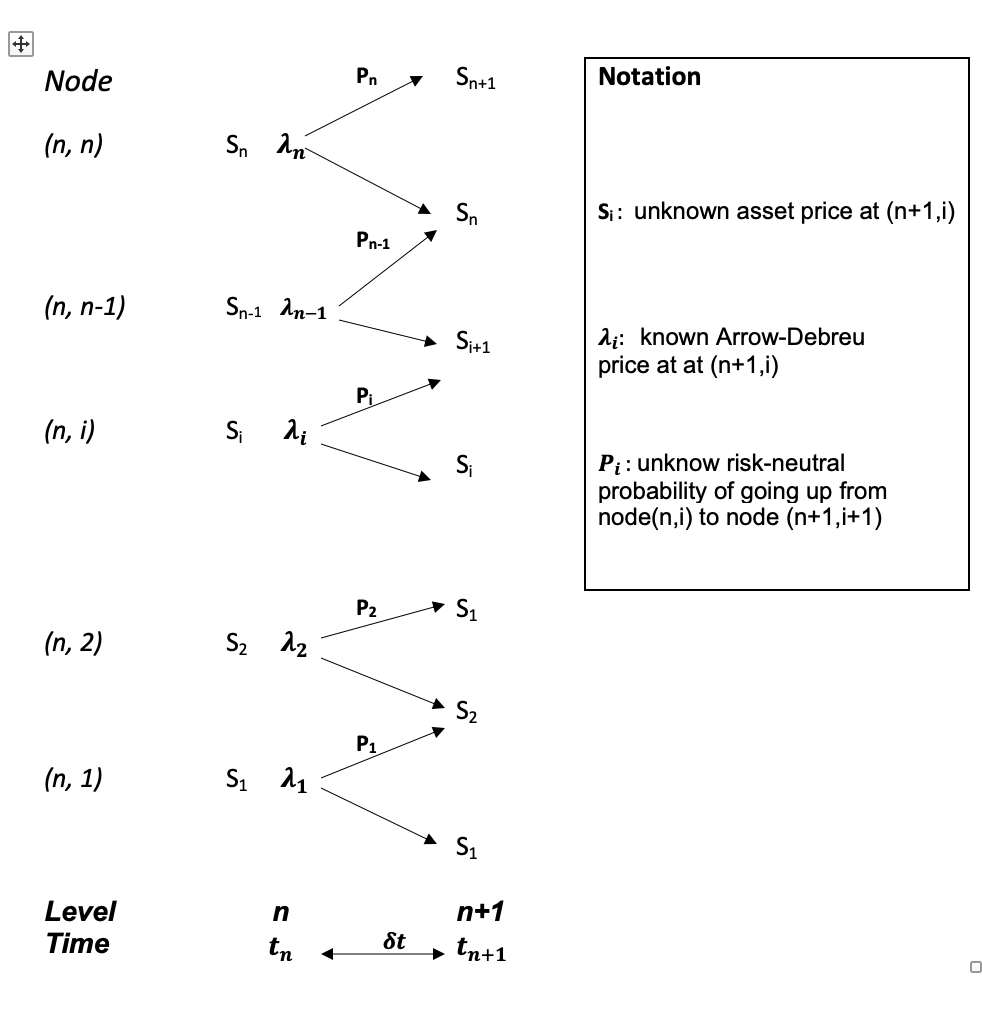
\includegraphics[width=0.5\columnwidth]{Figures/tree}
\decoRule
\caption{Constructing the $(n+1)^{th}$ Level of the Implied Tree}
\label{fig:tree}
\end{figure}
Under the risk-neutral assumption in the Binomial tree structure, the expected asset price one period ahead must agree with the forward price $F-i$:
\begin{equation}
\label{eqn:foward}
F_i = p_i S_{i+1} +(1-p_i)S_{i}
\end{equation}

Let $C(s_i, t_{n+1})$ and $P(s_i, t_{n+1})$ denote the market call and put prices struck today at $s_i$ and expiring at $t_{n+1}$ then those prices can be obtained by interpolating the smile structure at time $t_{n+1}$. Call option price with strike K, can be calculated by summing up the discounted payoff multiplied by the corresponding probabilities of reaching each note in the next step:
\begin{equation}
\label{eqn:call_tree}
C(K, t_{n+1}) = e^{-r \delta t} \sum_{j=1}^n {\lambda_j p_j +\lambda_{j+1}(1- p_{j+1})} \text{max} (S_{j+1}-K, 0)
\end{equation}
when the option is at the money, e.g $K= s_i$, Equation ~\ref{eqn:call_tree}, using the forward price equation, can be rewritten as:

\begin{equation}
\label{eqn:re_tree}
e^{r \delta t}C(s_i, t_{n+1}) =   \lambda_i p_i (S_{i+1}-s_i)+\sum_{j=1}^n \lambda_{j}(F_j- s_i)
\end{equation}

Since both $C(s_i, t_{n+1})$ and $F_i$ are known, $S_{i+1}$ and $p_i$ can be solved with Equation 
~\ref{eqn:foward} and Equation~\ref{eqn:re_tree}.

\begin{align}
\label{eqn:iterative}
S_{i+1} = \frac{S_i[e^{r\delta t}C(s_i, t_{n+1})-\sum_{j=1}^n \lambda_{j}(F_j- s_i)]-\lambda_i s_i(F_i-S_i) }{[e^{r\delta t} C(s_i, t_{n+1})-\sum_{j=1}^n \lambda_{j}(F_j- s_i)]-\lambda_i (F_i-S_i)}\\
p_i = \frac{F_i -S_i}{S_{i+1}-S_i}
\end{align}

Iteratively, in this manner, we can find the prices and 'up' and 'down' probabilities in each node above the centre of the tree given the known initial node.

In particular, if the number of the nodes in $n+1^{th}$ node is odd, then we set initial $S_i$ with $i=n/2 +1$ with the spot price $s_i$at the central node. Use equations in ~\ref{eqn:iterative} we can cover each node in upper half of the tree.  

if the number of the nodes in $n+1^{th}$ node is even, we start with the nodes just above and below the central level, $S_{i+1}$ and $S_i$ respectively. This two nodes need to satisfy the condition $S_i = \frac{s_i^2}{S_{i+1}}$. Together with Equation~\ref{eqn:call_tree} we have:
\begin{equation}
S_{i+1} = \frac{s_i[e^{r\delta} t C(s_i, t_{n+1})+\lambda_i s_i -\sum_{j=1}^n \lambda_{j}(F_j- s_i)]}{\lambda_i F_i - e^{r\delta t} C(s_i, t_{n+1})+\sum_{j=1}^n \lambda_{j}(F_j- s_i)} \quad\quad\quad for \quad i =n/2
\end{equation}
Similarly, we construct the lower part of the tree iteratively use:
\begin{equation}
S_{i} = \frac{S_{i+1}[e^{r\delta} t P(s_i, t_{n+1})-\sum_{j=1}^n \lambda_{j}(F_j- s_i)]+\lambda_i s_i(F_i-S_{i+1})}{[e^{r\delta t} P(s_i, t_{n+1})-\sum_{j=1}^n \lambda_{j}(F_j- s_i)]+\lambda_i (F_i-S_{i+1})} 
\end{equation}
Hence, the implied local volatility $\sigma(S,t)$ is reflected in the implied binomial tree.




%----------------------------------------------------------------------------------------


%----------------------------------------------------------------------------------------

%----------------------------------------------------------------------------------------


 
%\include{Chapters/Chapter5} 

%----------------------------------------------------------------------------------------
%	THESIS CONTENT - APPENDICES
%----------------------------------------------------------------------------------------

\appendix % Cue to tell LaTeX that the following "chapters" are Appendices

% Include the appendices of the thesis as separate files from the Appendices folder
% Uncomment the lines as you write the Appendices

%% Appendix A

\chapter{Frequently Asked Questions} % Main appendix title

\label{AppendixA} % For referencing this appendix elsewhere, use \ref{AppendixA}

\section{How do I change the colors of links?}

The color of links can be changed to your liking using:

{\small\verb!\hypersetup{urlcolor=red}!}, or

{\small\verb!\hypersetup{citecolor=green}!}, or

{\small\verb!\hypersetup{allcolor=blue}!}.

\noindent If you want to completely hide the links, you can use:

{\small\verb!\hypersetup{allcolors=.}!}, or even better: 

{\small\verb!\hypersetup{hidelinks}!}.

\noindent If you want to have obvious links in the PDF but not the printed text, use:

{\small\verb!\hypersetup{colorlinks=false}!}.

%\include{Appendices/AppendixB}
%\include{Appendices/AppendixC}

%----------------------------------------------------------------------------------------
%	BIBLIOGRAPHY
%----------------------------------------------------------------------------------------

\printbibliography[heading=bibintoc]

%----------------------------------------------------------------------------------------

\end{document}  
